\documentclass[10pt, a4paper,spanish]{article}
\usepackage[utf8]{inputenc}

\usepackage{hyperref}

\usepackage[T1]{fontenc}

\usepackage[hmarginratio=1:1,top=32mm,columnsep=20pt]{geometry}
\usepackage[hang, small,labelfont=bf,up,textfont=it,up]{caption}


\usepackage{graphicx}
\graphicspath{ {images/} }

\usepackage{abstract}
\renewcommand{\abstractnamefont}{\normalfont\bfseries}
\renewcommand{\abstracttextfont}{\normalfont\small\itshape}

\usepackage{titlesec}
\renewcommand\thesection{\Roman{section}}
\renewcommand\thesubsection{\Roman{subsection}}
\titleformat{\section}[block]{\large\scshape\centering}{\thesection.}{1em}{}
\titleformat{\subsection}[block]{\large}{\thesubsection.}{1em}{}


\usepackage{fancyhdr}
\pagestyle{fancy}
\fancyhead{}
\fancyfoot{}
\fancyhead[C]{ \today \ $\bullet$ Minería de Datos $\bullet$ Mapa Auto-organizado y Perceptrón Multicapa}
\fancyfoot[RO,LE]{\thepage}

%----------------------------------------------------------------------------------------
%	TITLE SECTION
%----------------------------------------------------------------------------------------

\title{\vspace{-15mm}\fontsize{24pt}{10pt}\selectfont\textbf{Mapa Auto-organizado y \\ Perceptrón Multicapa}} % Article title

\author{Sergio García Prado}
\date{\today}

%----------------------------------------------------------------------------------------

\begin{document}

	\maketitle % Insert title

	\thispagestyle{fancy} % All pages have headers and footers

%----------------------------------------------------------------------------------------
%	ABSTRACT
%----------------------------------------------------------------------------------------

	\begin{abstract}
		\noindent El trabajo consiste en la implementación de un Mapa Auto-organizado en el lenguaje Matlab, el cual se ha utilizado como "filtro" de entrada hacia Perceptrón Multicapa. Para realizar dichas pruebas se ha utilizado el MLP implementado en la biblioteca WEKA del lenguaje Java.
	\end{abstract}
%----------------------------------------------------------------------------------------
%	TEXT
%----------------------------------------------------------------------------------------

	\section{Introducción}

		\subsection{Mapa Auto-organizado}

			\paragraph{}
			Un mapa auto-organizado es un tipo de red neuronal artificial, que es entrenada usando aprendizaje no supervisado para producir una representación discreta del espacio de las muestras de entrada, llamado mapa. Los mapas auto-organizados son diferentes de otras redes neuronales artificiales, en el sentido que estos usan una función de vecindad para preservar las propiedades topológicas del espacio de entrada.

			\paragraph{}
			El modelo fue descrito por primera vez como una red neuronal artificial por el profesor finlandés Teuvo Kohonen, debido a lo cual en ocasiones son llamadas redes o mapas de Kohonen. Al igual que la mayoría de las redes neuronales artificiales, los SOMs operan en dos modos: entrenamiento y mapeo. En el entrenamiento construye el mapa usando ejemplos entrenantes, mientras que en el mapeo clasifica una nueva entrada.

			\paragraph{}
			Un mapa auto-organizado consiste en un conjunto de componentes llamadas nodos o neuronas. Asociado con cada neurona hay un vector de pesos, de la misma dimensión de los vectores de entrada, y una posición en el mapa. La configuración usual de las neuronas es un espacio regular de dos dimensiones, en una rejilla hexagonal o rectangular. Los mapas auto-organizados describen un mapeo de un espacio de mayor dimensión a uno de menor dimensión. El procedimiento para ubicar un vector del espacio de los datos en el mapa es encontrar la neurona con el vector de pesos más cercano (menor distancia métrica) al vector del espacio de los datos. El proceso de aprendizaje se lleva a cabo a través de la relación de vecindad entre neuronas, siendo afectadas tanto la de menor distancia a la entrada y las vecinas de la misma.


		\subsection{Perceptrón Multicapa}

			\paragraph{}
			El perceptrón multicapa es una red neuronal formada por múltiples capas, esto le permite resolver problemas que no son linealmente separables, lo cual es la principal limitación del perceptrón simple. El perceptrón multicapa puede ser total o localmente conectado. En el primer caso cada salida de una neurona de la capa "i" es entrada de todas las neuronas de la capa "i+1", mientras que en el segundo cada neurona de la capa "i" es entrada de una serie de neuronas (región) de la capa "i+1".

	\clearpage
	\section{Implementación}

		\paragraph{}
		La implementación consiste en el desarrollo de un mapa auto-organizado en el lenguaje Matlab, cuya salida de la fase no supervisada se ha introducido en un perceptrón multicapa. Para ello se ha utilizado el MLP que implementa la librería WEKA. Además se ha desarrollado la fase supervisada del mapa auto-organizado, por lo que se ha podido obtener una comparativa sobre las dos alternativas.

		\paragraph{}
		El conjunto de datos utilizado se corresponde a una codificación numérica de manuscritos que representan números del 0 al 9. Estos han sido codificados en 40 componentes, las cuales representan un tablero de 5 x 8 casillas. Existen dos ficheros, el primero contiene 270 muestras que serán utilizadas para entrenamiento y el segundo 70 para tareas de test y comprobación de resultados.



		\paragraph{}
		Podemos dividir la implementación realizada en las siguientes partes según la funcionalidad que aporta cada una:

		\subsection{Mapa auto-organizado}

			\paragraph{}
			El mapa auto-organizado implementado se ha probado con unas dimensiones de 12 x 8 neuronas, aunque este valor se puede modificar. También se han utilizado 50 épocas para la fase de aprendizaje no supervisado y un coeficiente de aprendizaje $\alpha_0$ de 25. Para la fase de aprendizaje supervisado se ha realizado un etiquetado por neuronas.

			\paragraph{}
			Lo primero que sucede al obtener los datos de entrada es la transformación de los mismos a un formato con el que se pueda trabajar con facilidad (dado que su distribución en los ficheros no sigue una estructura que facilite la realización de operaciones). Por tanto, se divide cada uno de los ficheros en 2 matrices, que representan las muestras por filas y, los atributos por columna en el caso del primero y la clase de cada muestra en la segunda matriz (realizando la tranformación apropiada de dimension 10 original a dimensión 1 convirtiéndolo en un número $n \in [0,9]$). Para que no surjan problemas de colisión en la fase de normalización se añade una nueva componente a todas las muestras cuyo valor es 1.

			\paragraph{}
			El siguiente paso es normalizar la matriz que contiene los atributos de entrada por filas para que no surjan problemas debido a la escala de los mismos. El último paso antes de comenzar con la fase no supervisada del algoritmo, se refiere a la inicialización de los pesos de las componentes de cada neurona (generados aleatoriamente en el rango $[-0.5, 0.5]$), que después son normalizados para poder aplicar en fases siguientes la propiedad del coseno para el cálculo de distancias.

			\begin{itemize}

				\item \textbf{Fase No Supervisada de SOM}: Consiste en el proceso de aproximación de los pesos de las neuronas inicializadas anteriormente hacia los valores cada componente de las muestras. Para ello, por cada muestra, se calcula la distancia a todas las neuronas del mapa para saber cuál es la más cercana. A esta neurona se la denomina \emph{ganadora} y será en torno a la cual se produzca el aprendizaje durante dicha iteracción. Lo siguiente es calcular el conjunto de neuronas que serán adaptadas (radio de vecindad). En este caso se ha decido utilzar una estructura cuadrada cuyo lado inicial es igual al lado de menor longitud del mapa. Este radio va decreciendo con el número de iteracciones hasta que solo se ve afectada la neurona ganadora. Seguidamente, se utiliza el coeficiente de aprendizaje (que depende de la época y es carácter decreciente), para tratar de "orientar" la dirección del vector de pesos de la neurona hacia la muestra correspondiente. En este caso se ha utilizado $\alpha(t) =  \frac{\alpha_0}{1 + t/P}$ siendo $t$ la época actual y $P$ el tamaño de muestras de la misma. Este proceso se realiza tantas veces como épocas se hayan fijado (50 por defecto en esta implementación).


				\item \textbf{Fase Supervisada de SOM}: La fase de aprendizaje supervisado consiste en el proceso de etiquetado de clases a cada neurona, ya que lo que se ha realizado hasta el momento es el cálculo para tratar de asemejar las neuronas del mapa a la entrada. Existen dos alternativas a la hora de realizar este proceso: etiquetado global y etiquetado por neuronas. En esta implementación se ha escogido el \textbf{etiquetado por neuronas} ya que aprovecha al máximo los calculos anteriores, haciendo uso de todas las neuronas (en el etiquetado global no se utilizan todas las disponibles por no ser ganadoras para ninguna muestra). Este proceso consiste en el cálculo de las distancias de todas las entradas a cada una de las neuronas etiquetandolas con la clase de la muestra más cercana a cada una de ellas.

			\end{itemize}



		\subsection{Perceptrón Multicapa}

			\paragraph{}


	\section{Resultados}

		\paragraph{}
		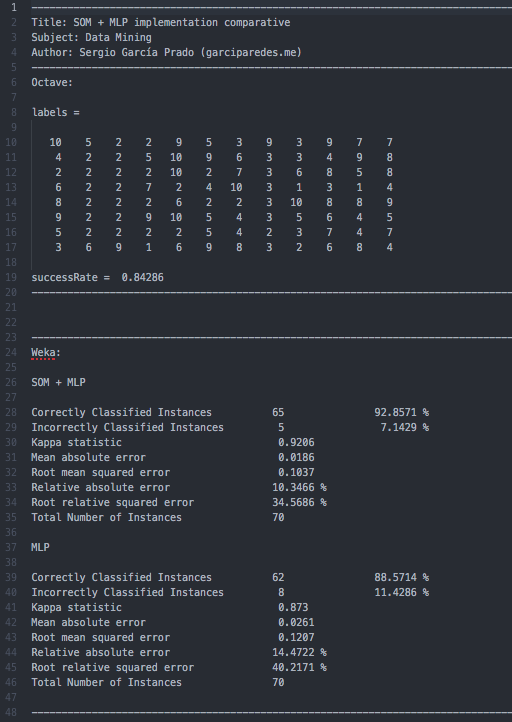
\includegraphics[width=\textwidth]{results}


\end{document}
